\documentclass{article}

\usepackage[numbers]{natbib}
% before loading neurips_2026

% The authors should use one of these tracks.
% Before accepting by the NeurIPS conference, select one of the options below.
% 0. "default" for submission
% \usepackage{neurips_2026}
% the "default" option is equal to the "main" option, which is used for the Main Track with double-blind reviewing.
% 1. "main" option is used for the Main Track
%  \usepackage[main]{neurips_2026}
% 2. "position" option is used for the Position Paper Track
%  \usepackage[position]{neurips_2026}
% 3. "eandd" option is used for the Evaluations & Datasets Track
 % \usepackage[eandd]{neurips_2026}
 % if you need to opt-in for a single-blind submission in the E&D track:
 %\usepackage[eandd, nonanonymous]{neurips_2026}
% 4. "creativeai" option is used for the Creative AI Track
%  \usepackage[creativeai]{neurips_2026}
% 5. "sglblindworkshop" option is used for the Workshop with single-blind reviewing
 % \usepackage[sglblindworkshop]{neurips_2026}
% 6. "dblblindworkshop" option is used for the Workshop with double-blind reviewing
%  \usepackage[dblblindworkshop]{neurips_2026}

% After being accepted, the authors should add "final" behind the track to compile a camera-ready version.
% 1. Main Track
 % \usepackage[main, final]{neurips_2026}
% 2. Position Paper Track
%  \usepackage[position, final]{neurips_2026}
% 3. Evaluations & Datasets Track
 % \usepackage[eandd, final]{neurips_2026}
% 4. Creative AI Track
%  \usepackage[creativeai, final]{neurips_2026}
% 5. Workshop with single-blind reviewing
%  \usepackage[sglblindworkshop, final]{neurips_2026}
% 6. Workshop with double-blind reviewing
%  \usepackage[dblblindworkshop, final]{neurips_2026}
% Note. For the workshop paper template, both \title{} and \workshoptitle{} are required, with the former indicating the paper title shown in the title and the latter indicating the workshop title displayed in the footnote.
% For workshops (5., 6.), the authors should add the name of the workshop, "\workshoptitle" command is used to set the workshop title.
% \workshoptitle{WORKSHOP TITLE}

% "preprint" option is used for arXiv or other preprint submissions
\usepackage[preprint]{neurips_2026}

% to avoid loading the natbib package, add option nonatbib:
   % \usepackage[nonatbib]{neurips_2026}

\usepackage[utf8]{inputenc} % allow utf-8 input
\usepackage[T1]{fontenc}    % use 8-bit T1 fonts
\usepackage{hyperref}       % hyperlinks
\usepackage{url}            % simple URL typesetting
\usepackage{booktabs}       % professional-quality tables
\usepackage{amsfonts}       % blackboard math symbols
\usepackage{nicefrac}       % compact symbols for 1/2, etc.
\usepackage{microtype}      % microtypography
\usepackage{xcolor}         % colors
\usepackage{amsmath}
\usepackage{graphicx}
\usepackage{cleveref}
\setlength{\textfloatsep}{\baselineskip}
\usepackage{multirow}
\usepackage{float}

% Note. For the workshop paper template, both \title{} and \workshoptitle{} are required, with the former indicating the paper title shown in the title and the latter indicating the workshop title displayed in the footnote. 
\title{When to Trust Imagination: Adaptive Action Execution for World Action Models}

% The \author macro works with any number of authors. There are two commands
% used to separate the names and addresses of multiple authors: \And and \AND.
%
% Using \And between authors leaves it to LaTeX to determine where to break the
% lines. Using \AND forces a line break at that point. So, if LaTeX puts 3 of 4
% authors names on the first line, and the last on the second line, try using
% \AND instead of \And before the third author name.


\author{
Rui Wang$^{1,*}$ \quad
Yue Zhang$^{2,*}$ \quad
Jiehong Lin$^2$ \quad
Kuncheng Luo$^3$ \\
\textbf{Jianan Wang}$^3$ \quad
\textbf{Zhongrui Wang}$^{1,\dagger}$ \quad
\textbf{Xiaojuan Qi}$^{2,\dagger}$ \\
$^1$Southern University of Science and Technology, Shenzhen, China \\
$^2$The University of Hong Kong, Hong Kong, China \\
$^3$Astribot, Shenzhen, China \\
\texttt{wangr2025@mail.sustech.edu.cn, u3009724@connect.hku.hk} \\
\texttt{mortimer.jh.lin@gmail.com, luo.kuncheng@astribot.com} \\
\texttt{jiananwang@astribot.com, wangzr@sustech.edu.cn, xjqi@eee.hku.hk} \\
$^*$Equal contribution \qquad $^\dagger$Corresponding authors
}


\begin{document}

\maketitle

\begin{abstract}
World Action Models (WAMs) have recently emerged as a promising paradigm for robotic manipulation by jointly predicting future visual observations and future actions. However, current WAMs typically execute a fixed number of predicted actions after each model inference, leaving the robot blind to whether the imagined future remains consistent with the actual physical rollout. In this work, we formulate adaptive WAM execution as a \emph{future--reality verification} problem: the robot should execute longer when the WAM-predicted future remains reliable, and replan earlier when reality deviates from imagination. To this end, we propose \emph{Future Forward Dynamics Causal Attention} (FFDC), a lightweight verifier that jointly reasons over predicted future actions, predicted visual dynamics, real observations, and language instructions to estimate whether the remaining action rollout can still be trusted. FFDC enables adaptive action chunk sizes as an emergent consequence of prediction--observation consistency, preserving the efficiency of long-horizon execution while restoring responsiveness in contact-rich or difficult phases. We further introduce Mixture-of-Horizon Training to improve long-horizon trajectory coverage for adaptive execution. Experiments on the RoboTwin benchmark and in the real world demonstrate that our method achieves a strong robustness--efficiency trade-off: on RoboTwin, it reduces WAM forward passes by 69.10\% and execution time by 34.02\%, while improving success rate by 2.54\% over the short-chunk baseline; in real-world experiments, it improves success rate by 35\%.

\end{abstract}

\section{Introduction}
\label{sec:introduction}

% Background (WAM)

Humans do not execute actions by blindly committing to a fixed future plan. Instead, we constantly predict how the world should evolve under our actions and compare this internal prediction with what we actually observe. When the predicted future remains consistent with reality, we can act smoothly over a long horizon; when the prediction deviates from observation, we immediately slow down, correct, or replan. A familiar example is missing a stair step: the body has already predicted the expected sensory feedback, and the sudden mismatch between expectation and reality creates an immediate warning signal. This prediction--observation comparison is central to robust physical interaction, especially when the world becomes uncertain, contact-rich, or difficult to model.

Recent World Action Models (WAMs) provide a promising computational analogue of this mechanism. Unlike conventional vision-language-action policies~\cite{shukor2025smolvla, black2024pi_0, black2025pi_, lv2025f1} that mainly generate actions from the current observation and instruction, WAMs jointly predict future visual observations and future actions~\citep{pai2025mimic, liang2025video, li2026causal, du2023learning, ye2024latent, guo2024prediction}. Through large-scale video-action pretraining, WAMs acquire spatiotemporal priors and physical dynamics knowledge, enabling stronger generalization to novel environments, unseen tasks, and new motion patterns. Recent studies~\citep{bi2025motus, li2025unified, zhu2025unified, ye2026gigaworld, ye2026world, yuan2026fast, beingh07} have demonstrated strong performance in zero-shot generalization, cross-environment transfer, and cross-embodiment learning. However, despite their ability to imagine how the world will evolve, current WAMs typically use their predicted future only to generate an action chunk, while the execution process itself remains largely blind to whether the imagined future is still consistent with the physical rollout.


% Challenges
This reveals a fundamental limitation in current WAM execution. At each inference step, a WAM predicts a chunk of future actions~\citep{zhao2023learning} and the robot executes a fixed number of them before querying the model again. Such fixed-size execution ignores the fact that the reliability of WAM imagination varies across tasks and across phases within a task. For simple and predictable dynamics, such as approaching or grasping a rigid cup, the WAM prediction may remain accurate over a long horizon; in this case, repeatedly calling the WAM after only a few actions wastes computation. In contrast, for deformable, contact-rich, or stochastic interactions, such as folding cloth or manipulating objects with complex contact, the predicted future can quickly become unreliable; in this case, blindly executing a long action chunk can cause failure. Therefore, the key challenge is not merely choosing a better chunk size, but deciding \emph{when the WAM's imagined future should still be trusted during physical execution}.

Existing adaptive execution methods for diffusion policies or VLA models mainly adjust action chunk length based on action uncertainty, entropy, or policy-side confidence~\citep{jing2025mixture, wang2026vla, liang2026adaptive, wang2026open, wu2026speedup}. However, these methods do not exploit the defining property of WAMs: the model predicts not only what action to take, but also what future visual observations should occur if the action rollout remains valid. This creates a new form of self-verification. During execution, the robot can compare the real observation with the WAM-predicted observation at the corresponding timestep and jointly reason over them with the action sequence to assess whether the remaining rollout is still compatible with reality. If the predicted visual dynamics, the real observation, and the planned actions remain causally consistent, the robot can continue executing the current chunk and avoid expensive WAM inference. Otherwise, the inconsistency becomes an early warning signal, and the robot should stop the current rollout and replan from the latest observation.


\begin{figure}[t]
  \centering
  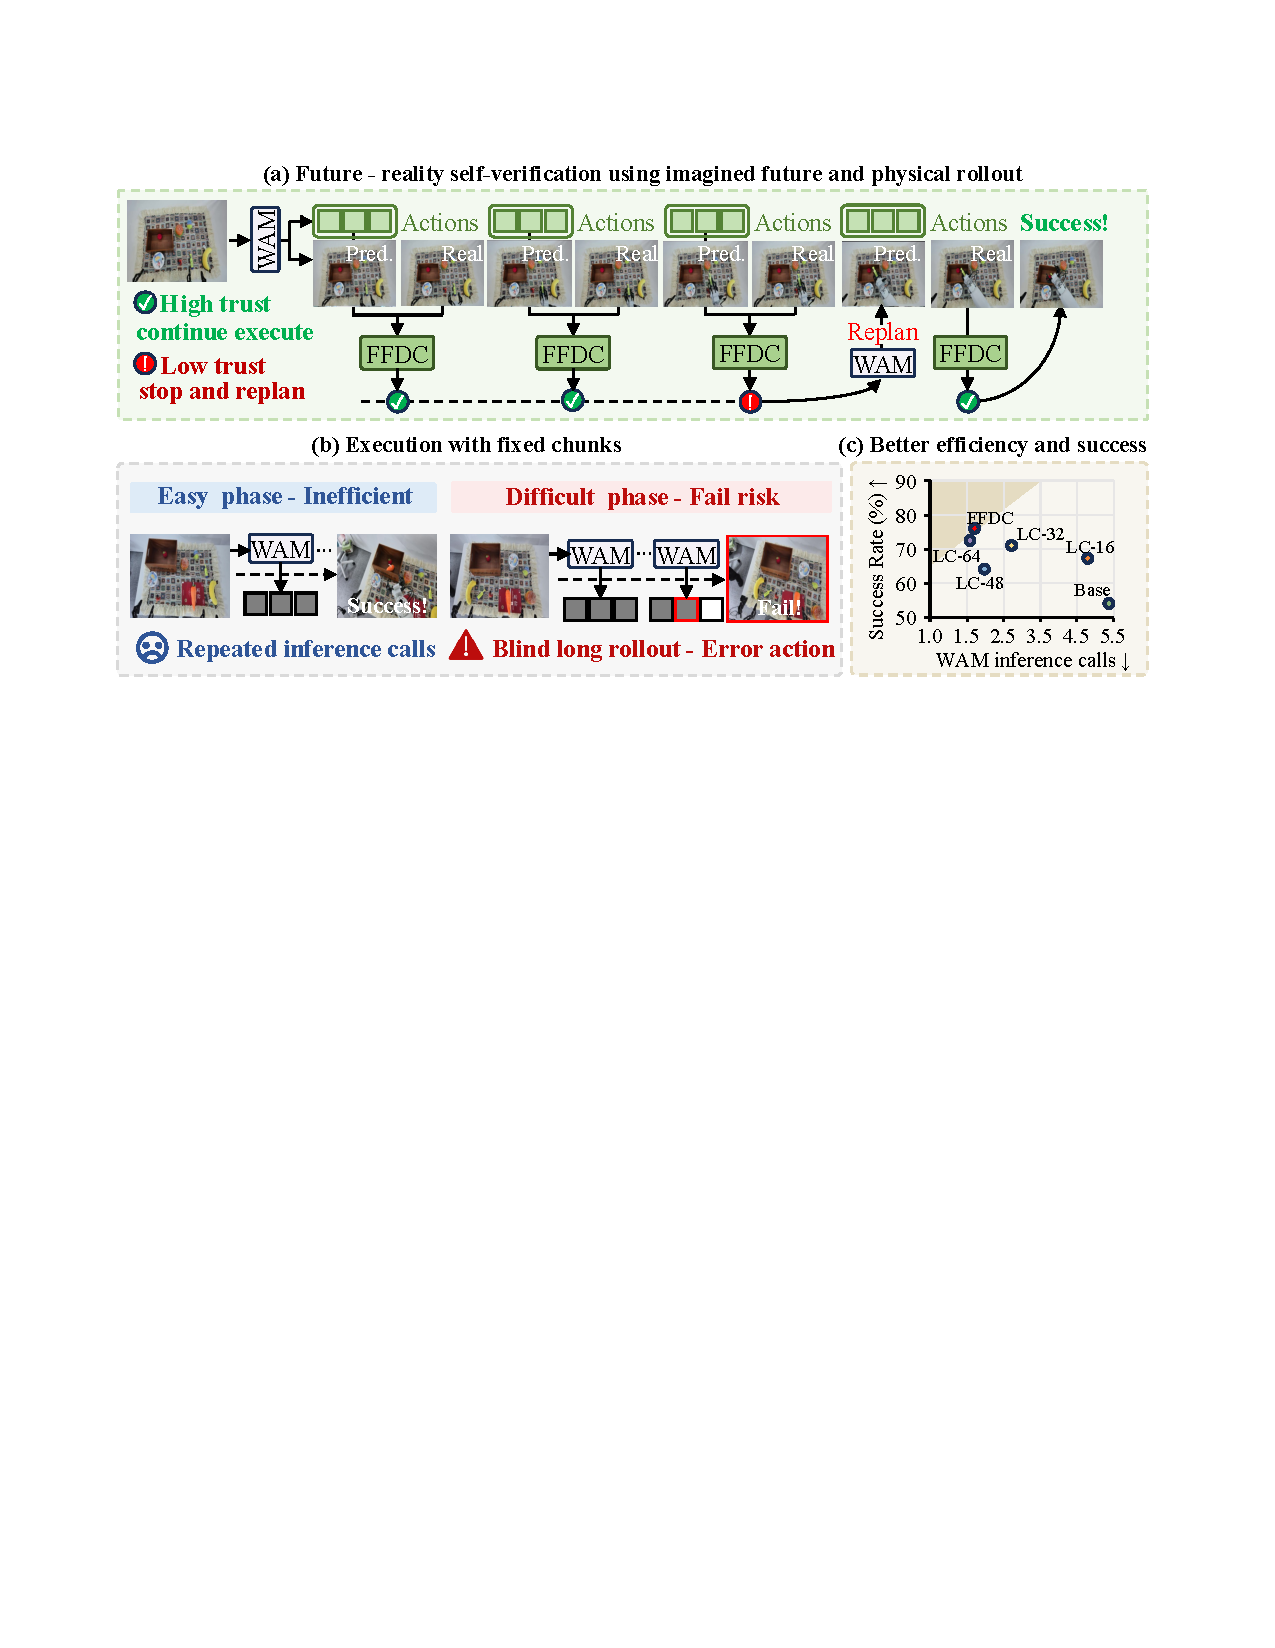
\includegraphics[width=1\linewidth, height=1\textheight, keepaspectratio,
                   trim=53 465 60 80, clip]{Fig1v2.pdf}
  \caption{FFDC enables adaptive trust in WAM imagination. (a) A WAM predicts future visual dynamics and an action chunk, and FFDC verifies during rollout whether the imagined future remains consistent with the real observation, planned actions, and instruction. Consistent predictions allow continued execution, while mismatches trigger replanning. (b) Fixed-size execution is inefficient in predictable phases and unreliable in difficult, contact-rich, or uncertain phases. (c) Scatter plot of success rate and task completion time on the RoboTwin benchmark. FFDC adapts execution length based on future--reality consistency, achieving a better robustness--efficiency trade-off.}
  \label{fig:fig1}
\end{figure}


% Our solution: 
Based on this insight, we propose an adaptive WAM execution framework that explicitly compares WAM imagination with physical rollout. The core module is \emph{Future Forward Dynamics Causal Attention} (FFDC), a lightweight verifier that estimates whether the remaining WAM-predicted action segment is still reliable. As shown in Fig.~\ref{fig:fig1} (a), the WAM predicts future visual dynamics and an action chunk, while FFDC verifies during execution whether the imagined future remains consistent with the real observation, planned actions, and language instruction. FFDC uses a structured attention mechanism to model the interaction between predicted vision and action, allowing it to detect task-critical mismatches and decide whether the remaining rollout can still be trusted. To equip FFDC with the ability to distinguish reliable imagined futures from deviations that require replanning, we construct a binary verification dataset using valid segments from demonstrations and successful rollouts, together with failure-prone segments from failed rollouts and synthetic action corruptions, and train it to predict the executability of the remaining action segment.

This design turns WAM execution from fixed open-loop rollout into adaptive future-aware control. In stable phases, FFDC allows the robot to trust the WAM's long-horizon imagination and execute more actions per inference, substantially reducing computation. In difficult phases, FFDC detects when the imagined future becomes unreliable and triggers replanning, improving robustness. As a result, the effective action chunk size is no longer a manually fixed hyperparameter, but an emergent consequence of future--reality consistency. The robot executes long when the world is predictable and short when reality deviates. As shown in Fig.~\ref{fig:fig1} (c), FFDC achieves the highest success rate while significantly reducing task completion time.

% Contributions
Our contributions are summarized as follows:
\begin{itemize}
    \item We formulate adaptive WAM execution as a \emph{future--reality verification} problem, where the WAM's predicted visual future is used to assess whether its remaining action rollout can still be trusted.
    \item We propose \emph{Future Forward Dynamics Causal Attention} (FFDC), a lightweight verifier that models temporally aligned causal interactions between predicted actions, predicted visual dynamics, real observations, and language instructions to detect unreliable future execution.
    \item We show that FFDC enables adaptive trust in WAM imagination: long execution in predictable phases to reduce inference cost, and short execution in difficult phases to improve robustness.
    \item Experiments on RoboTwin and in the real world validate our method. On RoboTwin, it reduces WAM forward passes by 69.10\% and execution time by 34.02\%, while improving success rate by 2.54\% over the short-chunk baseline; in the real world, it improves success rate by 35\%.
\end{itemize}

\section{Related work}

\paragraph{World action models.}
\label{sec:world action models}
World Action Models (WAMs) extend standard VLA policies by explicitly modeling how future observations evolve under actions through joint video-action generation~\citep{zhu2025unified,li2025unified, bi2025motus, ye2026world, li2026causal, yuan2026fast}. This formulation allows WAMs to capture multiple control-relevant distributions within a unified framework, including forward dynamics $p(o' \mid o, a)$, inverse dynamics $p(a \mid o, o')$, the marginal action distribution $p(a \mid o)$, and the marginal image distribution $p(o' \mid o)$ corresponding to video generation~\citep{zhu2025unified, bi2025motus, li2025unified}. Compared with VLAs that primarily model the action modality, WAMs benefit from dense supervision in video space, which provides rich information about contact, motion, and temporal scene evolution during execution~\citep{liu2026arflow, podell2023sdxl, tian2025pdfactor}.

Recent WAMs have demonstrated strong performance in zero-shot control, cross-environment transfer, and cross-embodiment learning. However, their future-prediction capability is often used mainly to improve representation learning or action generation. Since pixel-level video decoding is expensive, several works perform future video prediction mainly during training, while relying on latent world features or even skipping explicit future rollout at inference time for efficient policy
execution~\citep{yuan2026fast, ye2026gigaworld}. Although this improves efficiency, it leaves an important capability of WAMs underexplored: the predicted future can serve not only as an auxiliary training signal or action-generation context, but also as an internal expectation of how the physical world should evolve under the planned action sequence. This observation motivates us to revisit WAM execution from the perspective of whether the imagined future can be trusted during rollout.

\paragraph{Adaptive action execution.}
\label{sec:adaptive action execution}
A growing body of work studies adaptive action execution to mitigate the limitations of fixed open-loop rollout. Early interactive imitation learning methods reduce compounding errors by collecting corrective supervision or exposing the policy to recovery behaviors~\citep{ross2011reduction,
laskey2017dart}. Later approaches estimate uncertainty or execution risk during rollout, using signals such as ensemble disagreement, novelty, or diffusion loss to trigger expert intervention or corrective replanning~\citep{menda2019ensembledagger, hoque2021thriftydagger, lee2025diff}. More recently, adaptive execution has been explored for diffusion policies and VLA models, including multi-horizon action prediction~\citep{jing2025mixture}, entropy-based chunk-size selection~\citep{liang2026adaptive}, verifier-based replanning~\citep{wang2026open}, scheduler-based chunk downsampling
~\citep{wu2026speedup}, and online executable-horizon estimation~\citep{wang2026vla}. These methods show that fixed action chunks are often suboptimal and that execution length should vary with task state, uncertainty, or policy confidence.

However, existing adaptive execution methods are primarily designed for action-only policies or VLA models. Their decisions are typically based on the current observation, predicted actions, uncertainty, entropy, or auxiliary confidence, but they do not explicitly predict how the future scene should evolve under the planned actions. As a result, they cannot directly compare the policy's internal future expectation with the actual physical rollout. In contrast, WAMs jointly predict future visual dynamics and future actions, providing an imagined future that is temporally coupled with the action sequence. Our work studies adaptive execution in this WAM-specific setting. We formulate it as \emph{future--reality verification}: the robot compares WAM-predicted visual dynamics with real observations during execution to decide whether the remaining action sequence can still be trusted. This enables the effective action chunk size to expand when prediction and reality remain consistent and shrink when they diverge.


\section{Method}
\label{sec:method}
In this section, we present FFDC-WAM, a framework that combines low-frequency macro planning with high-frequency lightweight verification for efficient adaptive action execution by leveraging the joint video-action modeling capability of WAMs. We first introduce the standard action-chunking method in WAMs and adaptive action execution in Section~\ref{sec:preliminary}. We then present the architecture of FFDC-WAM in Section~\ref{sec:ffdc}, where a lightweight verifier performs high-frequency verification through a causal attention mechanism over visual and action modalities. Finally, in Section~\ref{sec:training strategy}, we describe the training strategies for the long-horizon WAM and the verifier module.

\subsection{Preliminary}
\label{sec:preliminary}
\paragraph{World action model with action chunking.}

We build on Motus~\citep{bi2025motus}, a world action model (WAM) that jointly predicts future actions and future visual observations conditioned on the current observation and language instruction. During training, the model is optimized with rectified flow-matching losses for both action and video prediction:
\begin{equation}
\mathcal{L}_{\text{WAM}} = \mathcal{L}_{\text{act}} + \mathcal{L}_{\text{vid}}.
\end{equation}

At inference time, given the current observation \(o_t\) and instruction \(\ell\), the WAM predicts a future action chunk and corresponding latent future visual tokens:
\begin{equation}
\label{eq:wampred}
(\hat{A}_{t+1:t+H}, \hat{O}_{t+1:t+H}) = \pi_\theta(o_t, \ell),
\end{equation}
where \(\hat{A}_{t+1:t+H}\) denotes the predicted action chunk of length \(H\), and \(\hat{O}_{t+1:t+H}\) denotes the predicted latent visual sequence.


\paragraph{Adaptive action execution.}
Standard action chunking executes the predicted chunk in an open-loop manner and replans only after all \(H\) actions are finished. While efficient, this fixed execution scheme can accumulate errors in dynamic or contact-rich scenarios.

To enable adaptive execution, we introduce a verifier \(\mu_\phi\) that decides whether the remaining predicted rollout is still trustworthy. After executing part of the current chunk, the verifier takes the latest observation, predicted future actions, predicted future visual tokens, and instruction as input:
\begin{equation}
e_t =
\mu_\phi\!\left(
o_t,\hat{A}_{t:t+k},\hat{O}_{t:t+k},\ell
\right),
\end{equation}
where \(e_t \in [0,1]\) is a confidence score. The robot continues execution if \(e_t \ge \tau\), and replans otherwise:
\begin{equation}
\label{eq:execution_decision}
\text{execute if } e_t \ge \tau,\qquad
\text{replan if } e_t < \tau,
\end{equation}
where \(\tau=0.5\) in this paper. The objective of adaptive execution is to retain the efficiency advantage of chunked inference while restoring responsiveness to execution failures and environmental changes.

\subsection{Future forward dynamics causal attention}
\label{sec:ffdc}

\begin{figure}[h]
  \centering
  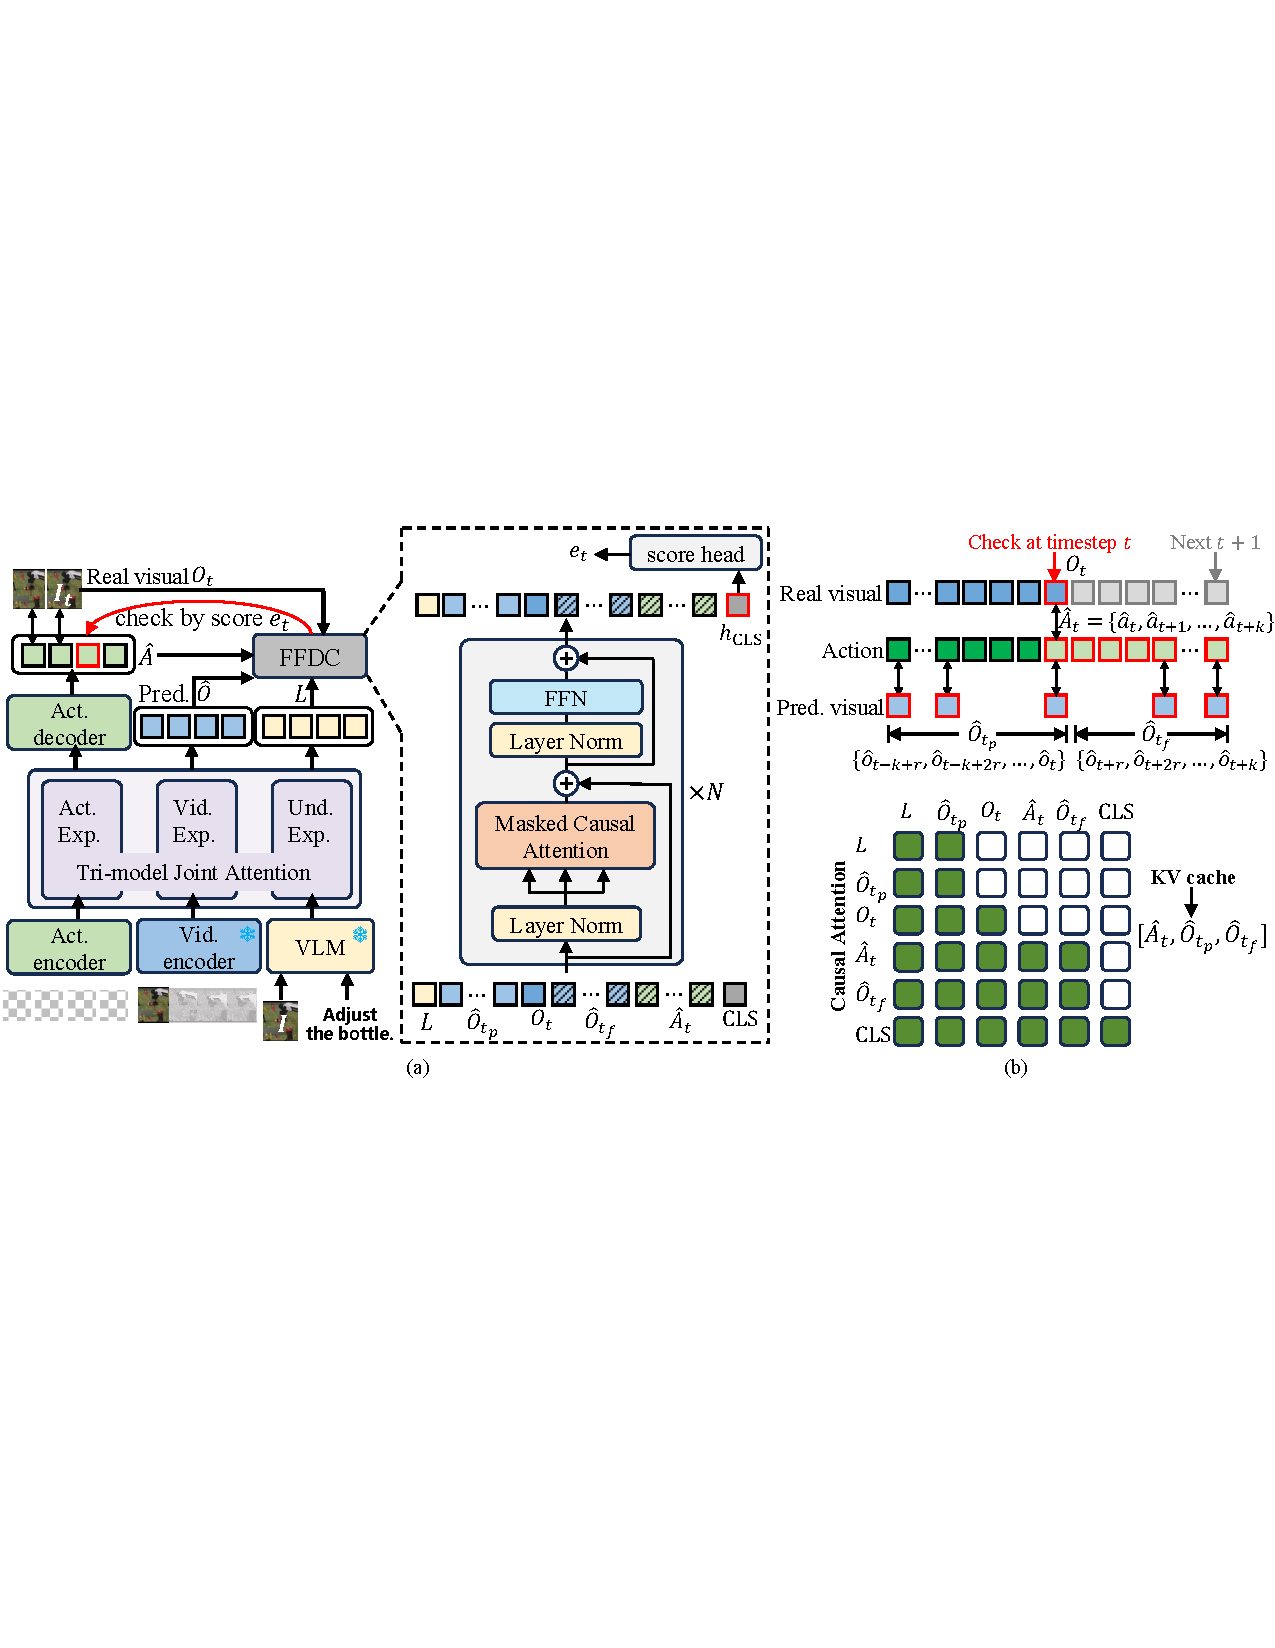
\includegraphics[width=1\linewidth, height=1\textheight, keepaspectratio,
                   trim=0 274 0 245, clip]{Fig2v2.pdf}
  \caption{Overview of the proposed FFDC-WAM. (a) Given the action sequence, predicted video tokens, and semantic tokens generated by WAM, the FFDC verifier outputs an execution confidence score for the remaining plan. (b) At each check step \(t\), FFDC performs structured causal attention, enforcing temporally aligned interaction between action and predicted visual dynamics.}
  \label{fig:fig2}
\end{figure}


\paragraph{Verifier architecture.}

To determine whether the remaining predicted plan is still reliable under the latest observation, we introduce a verifier based on \emph{Future Forward Dynamics Causal Attention} (FFDC). As illustrated in Fig.~\ref{fig:fig2} (a), each WAM inference produces a predicted action sequence \(\hat{A}\), the corresponding latent video tokens \(\hat{O}\), and the semantic tokens \(L\) from the Understanding expert.

At verification step \(t\), the verifier takes as input the current real observation tokens \(O_t\), the semantic tokens \(L\), the WAM-predicted historical video tokens \(\hat{O}_{t_p}\), the WAM-predicted future video tokens \(\hat{O}_{t_f}\), the future action segment \(\hat{A}_t\), and a learnable \texttt{[CLS]} token for global aggregation. The resulting verifier input sequence is
\begin{equation}
X_t = [L,\hat{O}_{t_p},O_t,\hat{O}_{t_f},\hat{A}_t,\texttt{[CLS]}].
\end{equation}

\paragraph{Future forward dynamics causal attention.}
To verify whether the next predicted action segment remains executable, we consider a horizon-\(k\) candidate rollout
\(
\hat{A}_t=[\hat{a}_t,\hat{a}_{t+1},\dots,\hat{a}_{t+k}]
\).
We also collect temporally aligned WAM-predicted visual tokens around timestep \(t\), including a past segment
\(
\hat{O}_{t_p}=[\hat{o}_{t-k+r},\hat{o}_{t-k+2r},\dots,\hat{o}_{t}]
\)
and a future segment
\(
\hat{O}_{t_f}=[\hat{o}_{t+r},\hat{o}_{t+2r},\dots,\hat{o}_{t+k}]
\),
where \(r\) is the action-to-video frequency ratio. In addition, we use instruction-conditioned semantic tokens \(L\) from the understanding expert and the latest real observation token \(O_t\).

A key design choice is that the WAM-predicted tokens, including past/future visual tokens \((\hat{O}_{t_p}, \hat{O}_{t_f})\), action tokens \(\hat{A}_t\), and understanding-expert tokens \(L\), are produced once after WAM inference and then stored as a \emph{KV cache}. During execution, the verifier only encodes the latest real observation \(O_t\) and performs lightweight attention against these cached tokens, which makes score computation efficient without rerunning the full WAM.

FFDC is implemented as an \(N\)-layer Transformer with a structured Boolean visibility matrix \(M\), where \(M(i,j)=1\) means token \(x_i\) can attend to token \(x_j\). The mask enforces causal interaction between future actions and future predicted dynamics. Specifically, besides attending to \(L\), \(O_t\), and \(\hat{O}_{t_p}\), each future visual token \(\hat{O}_{t_f}^{(j)}\) attends only to \(\{\hat{O}_{t_f}^{(\leq j)}, \hat{A}_{t}^{(\leq t+jr)}\}\), and each future action token attends only to \(\{\hat{O}_{t_f}^{(\leq j)}, \hat{A}_{t}^{(\leq t+jr)}\}\). To further reduce computation, this attention is applied with a local window over the temporally ordered future tokens, so each token interacts only with nearby aligned action/visual tokens rather than the full future sequence. This preserves temporal causality, avoids information leakage, and keeps the verifier lightweight.

Finally, a \texttt{[CLS]} token attends to the full visible sequence and aggregates the execution state into a compact representation. Its output is passed through an MLP head \(g_{\psi}\) to produce
\begin{equation}
z_t = g_{\psi}\!\left(\mathrm{FFDC}(X_t)_{\texttt{[CLS]}}\right),
\end{equation}
followed by
\begin{equation}
e_t = \sigma(z_t) \in [0,1],
\end{equation}
where a larger \(e_t\) indicates higher confidence that the future action segment \(\hat{A}_t\) remains valid under the latest real observation.

\subsection{Training strategy and dataset construction}
\label{sec:training strategy}
To improve trajectory coverage for long-horizon inference, we train WAM with a mixture-of-horizon sampling strategy. For an episode of length \(T\), we uniformly sample a conditioning timestep \(s \sim \mathcal{U}\{1,\dots,T\}\). Given horizon \(H\), the action and video indices are defined as \(\tau_i=\min(s+i,T)\), and \(\upsilon_j=\min(s+jr,T)\), where \(i=0,\dots,H-1\) and \(j=0,\dots,H/r-1\), which yield action and video sequences
\begin{equation}
A_s=[a_{\tau_0},\dots,a_{\tau_{H-1}}], \qquad
O_s=[o_{\upsilon_0},\dots,o_{\upsilon_{H/r-1}}].
\end{equation}
Out-of-range positions are padded by repeating the final valid action or frame. This allows late-stage states to serve as conditioning starts during training and reduces the bias toward early-episode prefixes.

For FFDC verifier training, we construct a binary dataset \(\mathcal{D}_{\mathrm{ver}}=\{(X,y)\}\), where \(X\) denotes the verifier input and \(y \in \{0,1\}\) indicates whether the future action segment is executable, with \(y=1\) for valid segments and \(y=0\) for failure-inducing ones. Positive samples are collected from demonstration data and a small number of successful rollouts. Negative samples are obtained from a small number of failed rollouts and from corrupted action segments synthesized from valid demonstrations. The data augmentation methods include temporal swap, gripper flip, late-stage Gaussian noise, and tail scaling. The temporal swap operator randomly swaps two pairs of actions within a horizon; gripper flip negates the designated gripper dimensions; late-stage Gaussian noise perturbs the second half of the sequence; and tail scaling shrinks a randomly sampled suffix by a random scale factor. Using the resulting dataset, the verifier is trained as a binary classifier with the loss

\begin{equation}
\mathcal{L}_{\mathrm{ver}}
=
-\Bigl[
y \log \sigma(z)
+
(1-y)\log \bigl(1-\sigma(z)\bigr)
\Bigr].
\end{equation}

\section{Experiments}
\label{sec:experiments}

\subsection{Experimental setups}
\label{sec:experiments setup}
We implement all models in PyTorch and adopt Motus~\cite{bi2025motus} as the WAM backbone; the complete system is referred to as \textbf{FFDC-WAM}. The backbone is trained on four NVIDIA A100 GPUs (80GB each), while the FFDC verifier is trained on a single A100 GPU. All evaluations are performed on one A100 GPU. We conduct online multi-task rollout evaluation in both the RoboTwin simulator~\cite{chen2025robotwin} and the real world. RoboTwin includes 50 manipulation tasks with diverse scenarios and randomized instructions, under both \emph{clean} and \emph{random} settings. The \emph{random} setting further introduces background variation, table clutter, height perturbation, and lighting changes, making it a challenging benchmark for testing generalization under distribution shift. In RoboTwin, each task is executed 100 times. For real-world evaluation, we use an Astribot S1 robot with 25 DoF~\cite{gao2025towards} and test two pick-and-place tasks.

\begin{figure}[H]
  \centering
  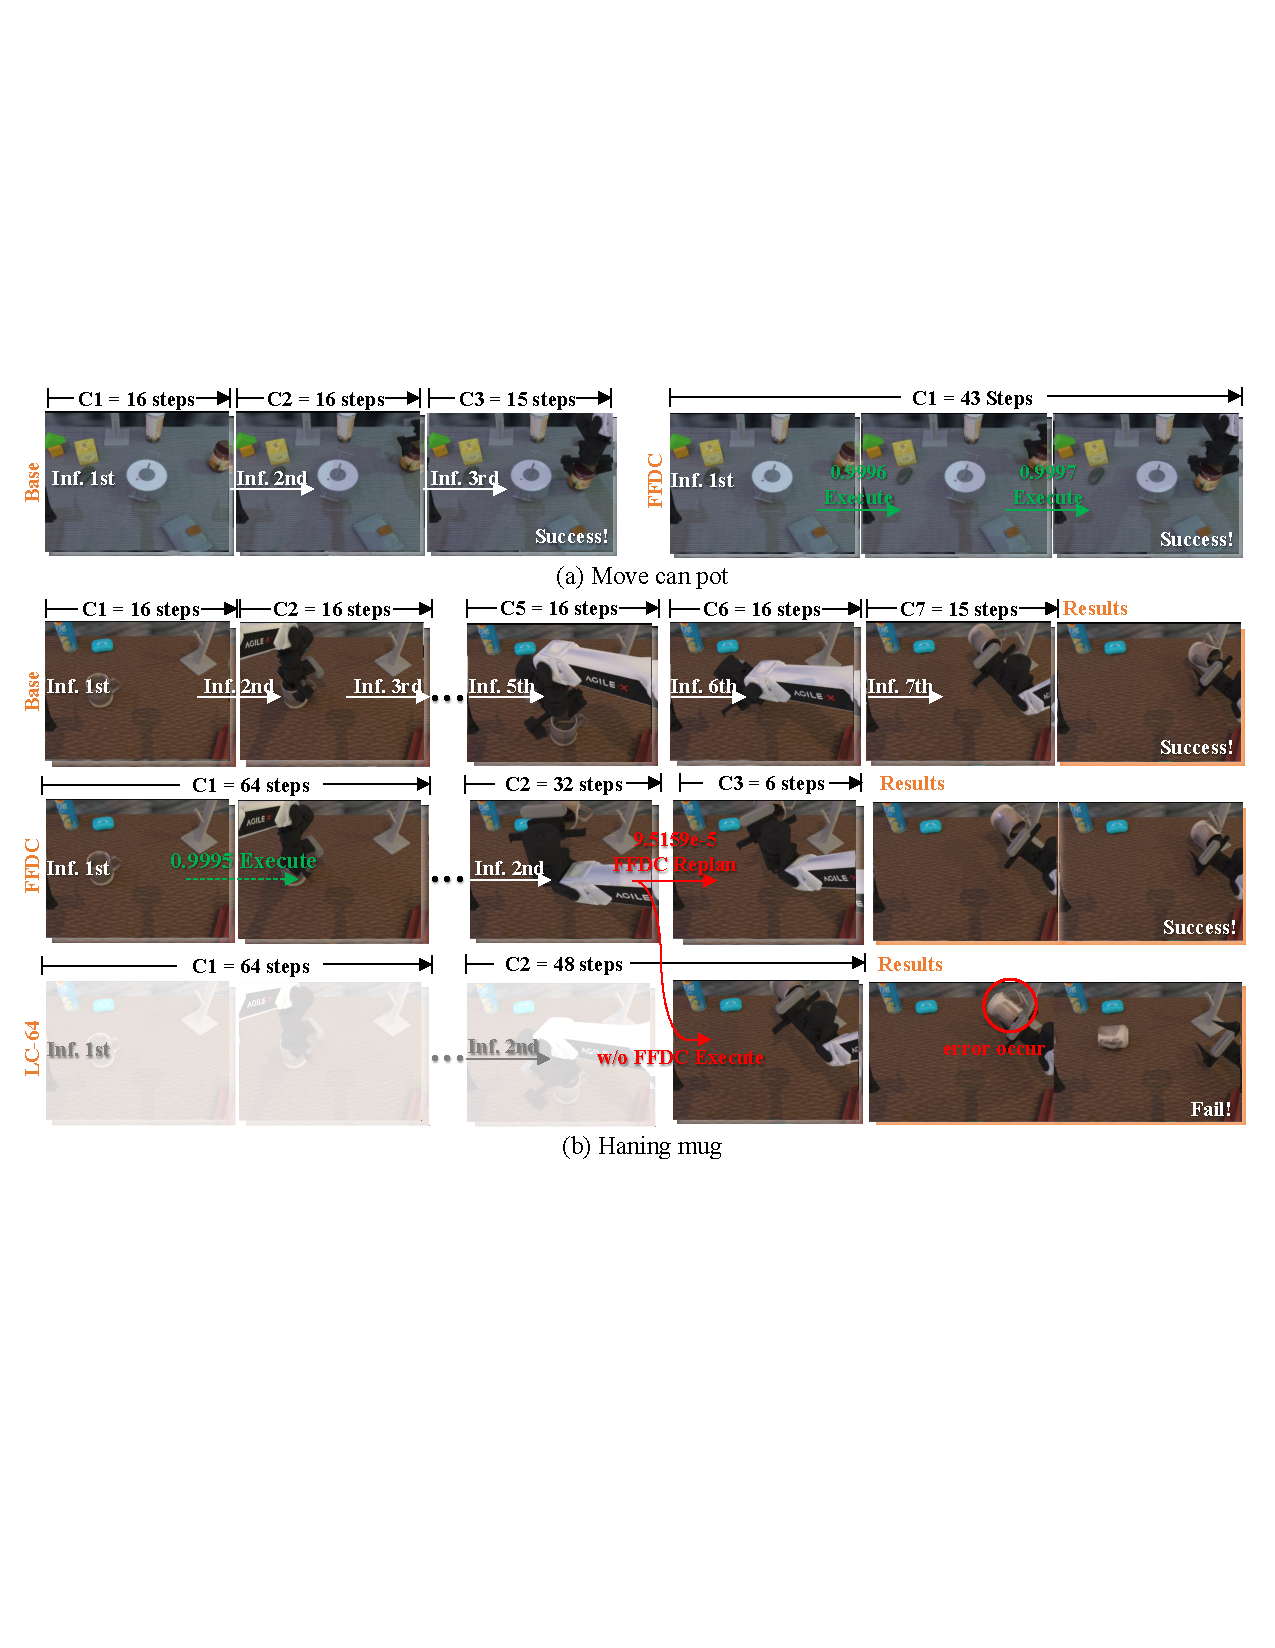
\includegraphics[width=1\linewidth, height=1\textheight, keepaspectratio,
                   trim=10 234 10 185, clip]{Fig3v3.pdf}
  \caption{Qualitative comparison of execution behaviors. (a) On the simple \textit{move can pot} task, \textbf{FFDC-WAM} completes the task with only one WAM inference, while \textbf{Base-Motus} requires three. The green scores indicate high FFDC confidence, allowing continued execution without replanning. (b) On a harder mug-hanging task, \textbf{FFDC-WAM} executes long-horizon actions during the predictable transport stage, but triggers replanning when confidence drops in the final precision-critical stage. In contrast, removing FFDC leads to direct open-loop execution of unreliable actions and eventual failure.}
  \label{fig:fig3}
\end{figure}

\subsection{Main results}
\label{sec:main_results}

\paragraph{Evaluation in simulation environment.}
We evaluate all methods on the RoboTwin benchmark~\cite{chen2025robotwin} under both \emph{clean} and \emph{random} settings, reporting success rate (SR) and average task completion time (T) over 50 tasks. Based on \textbf{Base-Motus}, we classify tasks with SR below 65\% as \emph{hard} and the rest as \emph{easy}; the hard tasks are \emph{Blocks Ranking Size}, \emph{Hanging Mug}, \emph{Place Mouse Pad}, \emph{Put Object in Cabinet}, and \emph{Scan Object}. Detailed per-task results are provided in the appendix. In Table~\ref{tab:main_results}, \textbf{Base-Motus} uses chunk size 16 for both training and testing. \textbf{LC-16/32/48/64} are long-chunk backbones trained with chunk size 64, while executing only the first 16, 32, 48, or 64 predicted actions at each step. \textbf{FFDC-WAM} is our adaptive execution method with the proposed verifier.


Overall, \textbf{FFDC-WAM} achieves the best balance between robustness and efficiency, with the highest average SR. On hard tasks, it substantially improves robustness over \textbf{Base-Motus}, raising SR from 54.20\% to 76.40\% on \emph{Rand.hard} and from 57.80\% to 76.00\% on \emph{Clean.hard}. On easy tasks, it runs much faster while maintaining comparable SR: completion time drops from 23.5s to 15.7s on \emph{Rand.easy} and from 20.4s to 12.9s on \emph{Clean.easy}. This shows that FFDC-WAM improves reliability when long-horizon prediction is hard to trust, and improves efficiency when prediction remains consistent with reality. Average model inference calls are reported in Table~\ref{tab:main_results}. Under the random setting, \textbf{FFDC-WAM} reduces model calls by 69.10\% compared with \textbf{Base-Motus} while completing the same tasks. Although fixed long-chunk baselines further reduce calls, they often sacrifice robustness on hard tasks. In contrast, \textbf{FFDC-WAM} adjusts inference frequency to task difficulty: it performs model inference more often on hard tasks, but stays close to \textbf{LC-64} on easy tasks. This confirms that FFDC improves efficiency by allocating model calls according to future--reality consistency, rather than blindly minimizing them.

\begin{table}[h]
\renewcommand{\arraystretch}{1.05}
\centering
\setlength{\tabcolsep}{3pt}
\caption{Main results on the RoboTwin benchmark, including success rate (SR), execution time (T), and average model inference calls.}
\label{tab:main_results}
\resizebox{\columnwidth}{!}{%
\begin{tabular}{@{}lcccccccccccccccccc@{}}
\toprule
\multirow{2}{*}{Case}
& \multicolumn{3}{c}{Base-Motus}
& \multicolumn{3}{c}{LC-16}
& \multicolumn{3}{c}{LC-32}
& \multicolumn{3}{c}{LC-48}
& \multicolumn{3}{c}{LC-64}
& \multicolumn{3}{c}{FFDC-WAM} \\
\cmidrule(lr){2-4}
\cmidrule(lr){5-7}
\cmidrule(lr){8-10}
\cmidrule(lr){11-13}
\cmidrule(lr){14-16}
\cmidrule(lr){17-19}
& SR(\%) & T(s) & Calls
& SR(\%) & T(s) & Calls
& SR(\%) & T(s) & Calls
& SR(\%) & T(s) & Calls
& SR(\%) & T(s) & Calls
& SR(\%) & T(s) & Calls \\
\midrule
Rand.hard
& 54.20 & 33.0 & 7.73
& 67.40 & 29.4 & 6.68
& 71.60 & 21.2 & 3.55
& 65.00 & 19.0 & 2.59
& 73.00 & 16.5 & 1.92
& \textbf{76.40} & 20.5 & 2.34 \\
Clean.hard
& 57.80 & 29.5 & 7.71
& 64.40 & 26.7 & 6.84
& 70.60 & 18.3 & 3.56
& 67.40 & 16.1 & 2.52
& 74.60 & 13.9 & 1.88
& \textbf{76.00} & 18.8 & 2.60 \\
Rand.easy
& 89.16 & 23.5 & 5.22
& 85.58 & 51.4 & 4.55
& 88.64 & 16.0 & 2.57
& 88.49 & 13.9 & 1.72
& 88.89 & 13.3 & 1.52
& \textbf{89.51} & 15.7 & 1.62 \\
Clean.easy
& \textbf{90.98} & 20.4 & 5.22
& 86.82 & 18.3 & 4.57
& 89.38 & 13.4 & 2.57
& 89.73 & 11.4 & 1.70
& 90.00 & 10.7 & 1.50
& 90.33 & 12.9 & 1.62 \\
\midrule
Rand.avg
& 85.66 & 24.4 & 5.47
& 83.76 & 22.0 & 4.76
& 86.94 & 16.5 & 2.67
& 86.14 & 14.4 & 1.81
& 87.26 & 13.6 & 1.56
& \textbf{88.20} & 16.1 & 1.69 \\
Clean.avg
& 87.66 & 21.3 & 5.47
& 84.58 & 19.1 & 4.80
& 87.50 & 13.8 & 2.67
& 87.50 & 11.8 & 1.79
& 88.46 & 11.1 & 1.54
& \textbf{88.90} & 13.5 & 1.72 \\
\bottomrule
\end{tabular}%
}
\end{table}

% \paragraph{Qualitative Visualization Analysis.}
To better understand this difficulty-aware behavior, we visualize execution in Fig.~\ref{fig:fig3} by comparing \textbf{Base-Motus} and \textbf{FFDC-WAM} on two representative tasks, where \(C_1, C_2, \ldots\) denote the executed action chunks. In Fig.~\ref{fig:fig3} (a), \textit{move can pot} is a simple task with simple dynamics. \textbf{Base-Motus} requires three WAM inferences due to fixed short-horizon execution, whereas \textbf{FFDC-WAM} completes the task with only one. The consistently high FFDC scores indicate that the predicted future remains reliable, allowing continued execution without replanning.

In Fig.~\ref{fig:fig3} (b), \textit{hanging mug} is more challenging and requires precise feedback-driven control. \textbf{Base-Motus} succeeds, but needs seven WAM inferences. \textbf{FFDC-WAM} instead behaves adaptively: it executes long chunks in the predictable transport stage, then switches to frequent replanning in the final precision-critical hanging stage when FFDC confidence drops. By contrast, directly executing the same long chunk without FFDC leads to accumulated error and eventual failure. This comparison highlights the key advantage of FFDC: reducing unnecessary model calls when prediction is reliable, while triggering timely replanning when it is not.



\paragraph{Real-world experiments.}
Real-world results are shown in Table~\ref{tab:real_exp}, with qualitative examples in Fig.~\ref{fig:fig4}. Compared with \textbf{LC-16}, \textbf{FFDC-WAM} improves the average success rate from 45\% to 80\% on both tasks. As illustrated in Fig.~\ref{fig:fig4}, this gain comes from FFDC's ability to detect execution drift online and trigger replanning when the real scene deviates from the predicted rollout: in both the banana and carrot tasks, \textbf{FFDC-WAM} alternates between execution and replanning and eventually succeeds, whereas \textbf{LC-16} continues open-loop execution without such verification and fails after error accumulation. This also explains the slightly higher execution time and model calls of \textbf{FFDC-WAM} (28.1s and 16 on average) than \textbf{LC-16} (25.6s and 14): in real-world settings, perception noise, actuation error, and contact uncertainty make future--reality consistency less reliable, so FFDC spends additional computation on online correction, which substantially improves robustness.

\begin{figure}[h]
  \centering
  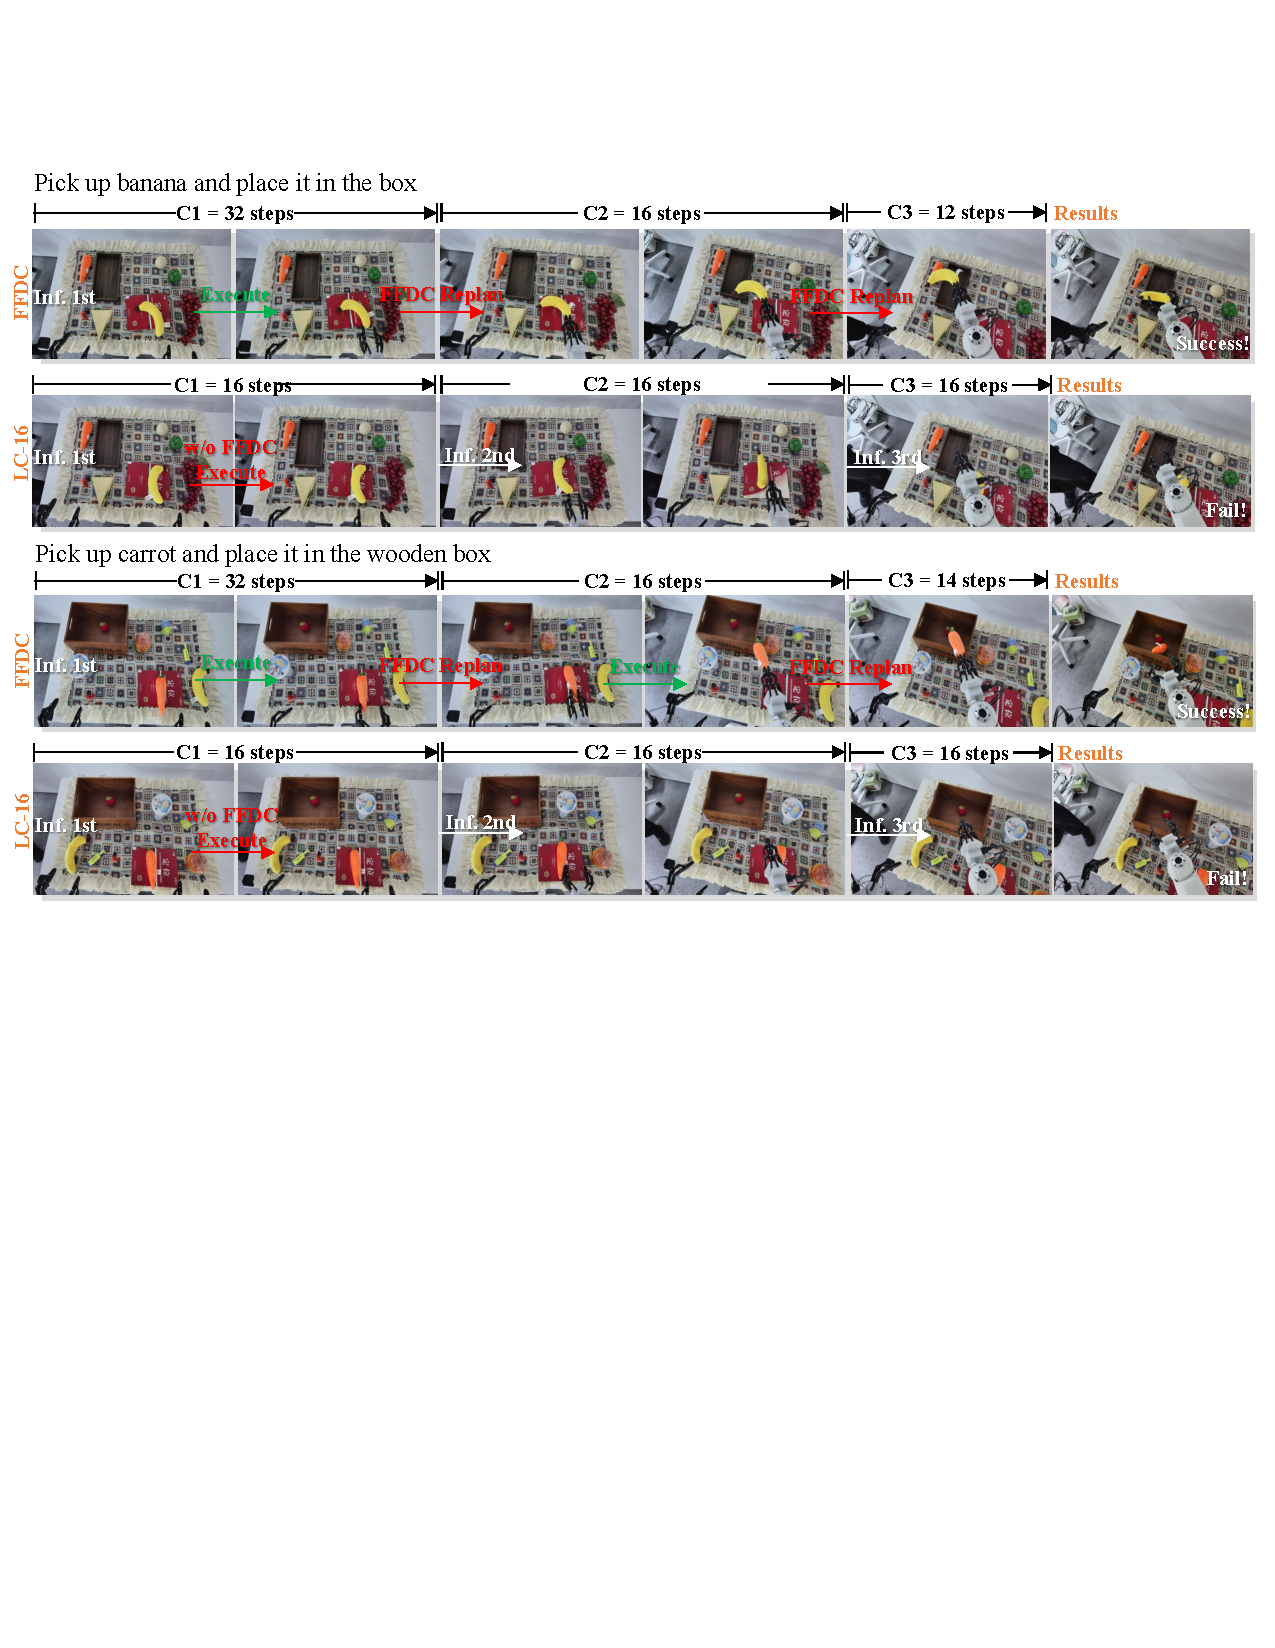
\includegraphics[width=1\linewidth, height=1\textheight, keepaspectratio,
                   trim=5 360 0 80, clip]{Fig4v1.pdf}
  \caption{Qualitative examples in real world.}
  \label{fig:fig4}
\end{figure}

\begin{table}[h]
\centering
\caption{Results on real-world tasks.}
\label{tab:real_exp}
\setlength{\tabcolsep}{2pt}
\renewcommand{\arraystretch}{0.8}
\begin{tabular}{lcccccc}
\toprule
\multirow{2}{*}{Task} 
& \multicolumn{3}{c}{LC-16} 
& \multicolumn{3}{c}{FFDC-WAM} \\
\cmidrule(lr){2-4} \cmidrule(lr){5-7}
& SR (\%) & T (s) & Calls & SR (\%) & T (s) & Calls \\
\midrule
pick banana and place & 50 & 25.6 & 14 & \textbf{80} & 26.7 & 15 \\
pick carrot and place & 40 & 25.6 & 14 & \textbf{80} & 29.5 & 17 \\
\midrule
Average & 45 & 25.6 & 14 & \textbf{80} & 28.1 & 16 \\
\bottomrule
\end{tabular}
\end{table}


\subsection{Ablation study}
\label{sec:ablation}
FFDC uses four inputs: predicted future actions, predicted visual tokens, the current real observation, and the language instruction. To evaluate their roles, we remove one input at a time and test on the hard-task subset of RoboTwin. In Table~\ref{tab:ablation_results}, \textbf{w/o Und}, \textbf{w/o Pred}, \textbf{w/o Real}, and \textbf{w/o Action} denote removing language, predicted visuals, real observation, and predicted actions, respectively.

The full model achieves the best overall performance, with the highest average success rate (76.4\%) and the lowest average completion time (20.5s). Removing any input lowers the average success rate, showing that reliable confidence estimation benefits from jointly modeling the imagined future, the current real state, the intended action rollout, and the task instruction. Among all variants, removing predicted visual tokens causes the largest drop in average success rate, from 76.4\% to 71.6\%, indicating that imagined future observations are the most informative signal for judging whether the rollout remains trustworthy. Removing the real observation also leads to a clear drop (72.4\%), confirming the importance of comparing predicted future dynamics against the actual current state. Removing action input reduces the average success rate to 73.4\%, showing that the predicted control sequence provides complementary information beyond visual prediction alone. Removing language conditioning causes a smaller but still consistent drop to 74.8\%, suggesting that task semantics further help FFDC assess rollout validity. Task-wise, the full model performs best on \textit{BlkRank}, \textit{HangMug}, and \textit{PutCab}, ties for best on \textit{PlacePad}, and remains competitive on \textit{ScanObj}, demonstrating that the complete FFDC design is the most robust overall.

\begin{table}[h]
\renewcommand{\arraystretch}{1.1}
\centering
\setlength{\tabcolsep}{0.8pt}
\caption{Ablation study results.}
\label{tab:ablation_results}
\resizebox{\columnwidth}{!}{%
\begin{tabular}{@{}lccccccccccccccc@{}}
\toprule
\multirow{2}{*}{Task}
& \multicolumn{3}{c}{w/o Und}
& \multicolumn{3}{c}{w/o Pred}
& \multicolumn{3}{c}{w/o Real}
& \multicolumn{3}{c}{w/o Action}
& \multicolumn{3}{c}{FFDC-WAM} \\
\cmidrule(lr){2-4}
\cmidrule(lr){5-7}
\cmidrule(lr){8-10}
\cmidrule(lr){11-13}
\cmidrule(lr){14-16}
& SR (\%) & T (s) & Calls
& SR (\%) & T (s) & Calls
& SR (\%) & T (s) & Calls
& SR (\%) & T (s) & Calls
& SR (\%) & T (s) & Calls \\
\midrule
BlkRank  & 91.0 & 26.1 & 3.34 & 85.0 & 24.9 & 3.11 & 86.0 & 27.8 & 3.70 & 90.0 & 25.5 & 3.31 & \textbf{93.0} & 25.3 & 3.27 \\
HangMug  & 37.0 & 29.2 & 4.16 & 32.0 & 27.8 & 4.03 & 38.0 & 27.3 & 3.92 & 33.0 & 28.9 & 4.24 & \textbf{44.0} & 27.5 & 3.96 \\
PlacePad & 86.0 & 12.5 & 1.23 & 84.0 & 12.4 & 1.24 & 87.0 & 12.3 & 1.20 & \textbf{88.0} & 13.1 & 1.43 & \textbf{88.0} & 12.4 & 1.27 \\
PutCab   & 72.0 & 26.6 & 3.49 & 71.0 & 21.9 & 2.01 & 68.0 & 21.7 & 2.00 & 69.0 & 22.1 & 2.00 & \textbf{73.0} & 21.7 & 2.00 \\
ScanObj  & \textbf{88.0} & 16.0 & 1.25 & 86.0 & 16.8 & 1.36 & 83.0 & 15.9 & 1.23 & 87.0 & 15.6 & 1.22 & 84.0 & 15.7 & 1.20 \\
\midrule
Average  & 74.8 & 22.1 & 2.69 & 71.6 & 20.8 & 2.35 & 72.4 & 21.0 & 2.41 & 73.4 & 21.0 & 2.44 & \textbf{76.4} & 20.5 & 2.34 \\
\bottomrule
\end{tabular}%
}
\end{table}


\section{Conclusion}
Inspired by how humans compare predicted future feedback with actual observation during physical interaction, we reformulate adaptive WAM execution as a \emph{future--reality verification} problem. Instead of using a fixed execution horizon, our method asks a more fundamental question: \emph{whether the WAM's imagined future can still be trusted during rollout}. To this end, we propose \textbf{FFDC-WAM}, where the lightweight \emph{Future Forward Dynamics Causal Attention} (FFDC) verifier jointly models temporally aligned interactions among predicted future actions, predicted visual dynamics, real observations, and language instructions to detect unreliable future execution.

This design enables adaptive trust in WAM imagination: the robot can continue execution when the predicted future remains reliable, and trigger replanning once future--reality consistency breaks down. In this way, FFDC-WAM moves WAM execution beyond fixed-horizon chunking toward a more principled reliability-aware control strategy, improving both efficiency and robustness across simulation and real-world settings. More broadly, our results suggest that the key to effective WAM deployment is not selecting a single execution length, but endowing the system with the ability to verify its own imagined future online. A current limitation is that FFDC is trained with binary supervision derived from successful, failed, and synthetically corrupted segments, which may not cover the full diversity of real-world execution deviations. Extending the verifier to learn from richer failure modes and more diverse real-world data is an important direction for future work.

\medskip
{
\small
\bibliographystyle{plainnat}
\bibliography{references}
}


%%%%%%%%%%%%%%%%%%%%%%%%%%%%%%%%%%%%%%%%%%%%%%%%%%%%%%%%%%%%

\appendix

\section{Technical appendices and supplementary material}
\label{appendix}

\subsection{Limitations}
\label{sec:limitations}
The current FFDC design adopts a relatively lightweight mechanism to model the relationship among predicted visual features, predicted actions, current observations, and language instructions. Although this design is efficient and effective in our experiments, it remains necessary to further explore the trade-off between the parameter scale of the FFDC module and its verification capability. In addition, the current method adopts a fixed detection threshold of 0.5 for FFDC-based execution decisions. A more systematic study of how the threshold affects the trade-off between robustness and efficiency may further improve performance. 


\subsection{Additional experimental results}
Results on hard tasks are shown in \cref{tab:hard_results}. Results on easy tasks under the random setting are shown in \cref{tab:easy_random_results}, and results on easy tasks under the clean setting are shown in \cref{tab:easy_clean_results}. Here, SR denotes success rate, and T denotes duration in seconds.

\begin{table}[h]
\renewcommand{\arraystretch}{1}
\centering
\setlength{\tabcolsep}{1.25pt}
\caption{Results on hard tasks.}
\label{tab:hard_results}
\begin{tabular}{@{}lcccccccccccc@{}}
\toprule
\multirow{2}{*}{Task}
& \multicolumn{2}{c}{Base-Motus}
& \multicolumn{2}{c}{LC-16}
& \multicolumn{2}{c}{LC-32}
& \multicolumn{2}{c}{LC-48}
& \multicolumn{2}{c}{LC-64}
& \multicolumn{2}{c}{FFDC-WAM} \\
\cmidrule(lr){2-3}
\cmidrule(lr){4-5}
\cmidrule(lr){6-7}
\cmidrule(lr){8-9}
\cmidrule(lr){10-11}
\cmidrule(lr){12-13}
& SR (\%) & T (s)
& SR (\%) & T (s)
& SR (\%) & T (s)
& SR (\%) & T (s)
& SR (\%) & T (s)
& SR (\%) & T (s) \\
\midrule
BlkRank rand.  & 62 & 49.1 & 66 & 43.1 & 78 & 30.0 & 62 & 26.7 & 89 & 21.4 & \textbf{93} & 25.3 \\
BlkRank clean  & 78 & 40.3 & 65 & 40.9 & 78 & 26.2 & 63 & 21.5 & 83 & 18.4 & \textbf{84} & 25.0 \\
HangMug rand.  & 38 & 36.2 & 42 & 31.8 & 35 & 24.6 & 26 & 22.0 & 32 & 18.9 & \textbf{44} & 27.5 \\
HangMug clean  & 27 & 30.8 & 27 & 29.5 & 23 & 22.2 & 21 & 19.7 & 25 & 16.7 & \textbf{30} & 26.5 \\
PlacePad rand. & 64 & 23.5 & 76 & 19.9 & 85 & 13.7 & 86 & 11.5 & 87 & 10.4 & \textbf{88} & 12.4 \\
PlacePad clean & 58 & 28.2 & 80 & 18.9 & 85 & 11.5 & 89 & 8.0 & 93 & 7.4 & \textbf{94} & 10.1 \\
PutCab rand.   & 53 & 32.5 & 67 & 29.7 & 67 & 21.0 & 66 & 18.7 & 72 & 17.9 & \textbf{73} & 21.7 \\
PutCab clean   & 62 & 29.3 & 60 & 26.1 & 76 & 18.2 & 73 & 16.2 & \textbf{81} & 16.0 & 80 & 19.2 \\
ScanObj rand.  & 54 & 23.9 & 86 & 22.6 & \textbf{93} & 16.7 & 85 & 16.0 & 85 & 13.7 & 84 & 15.7 \\
ScanObj clean  & 64 & 18.7 & 90 & 18.1 & 91 & 13.3 & 91 & 15.1 & 91 & 11.2 & \textbf{92} & 13.2 \\
\midrule
Average   & 56.0 & 31.3 & 65.9 & 28.1 & 71.1 & 19.7 & 66.2 & 17.5 & 73.8 & 15.2 & \textbf{76.2}  & 19.7 \\
\bottomrule
\end{tabular}
\end{table}

\begin{table}[t]
\renewcommand{\arraystretch}{1}
\centering
\setlength{\tabcolsep}{1.5pt}
\caption{Results on easy tasks under random environment setting.}
\label{tab:easy_random_results}
\begin{tabular}{@{}lcccccccccccc@{}}
\toprule
\multirow{2}{*}{Task}
& \multicolumn{2}{c}{Base-Motus}
& \multicolumn{2}{c}{LC-16}
& \multicolumn{2}{c}{LC-32}
& \multicolumn{2}{c}{LC-48}
& \multicolumn{2}{c}{LC-64}
& \multicolumn{2}{c}{FFDC-WAM} \\
\cmidrule(lr){2-3}
\cmidrule(lr){4-5}
\cmidrule(lr){6-7}
\cmidrule(lr){8-9}
\cmidrule(lr){10-11}
\cmidrule(lr){12-13}
& SR(\%) & T(s)
& SR(\%) & T(s)
& SR(\%) & T(s)
& SR(\%) & T(s)
& SR(\%) & T(s)
& SR(\%) & T(s) \\
\midrule
AdjBottle      & 87.0 & 15.5 & 98.0 & 14.7 & 98.0 & 12.2 & \textbf{99.0} & 9.6 & 98.0 & 9.7 & 98.0 & 11.2 \\
BeatBlock      & 90.0 & 15.4 & \textbf{96.0} & 15.2 & 92.0 & 12.1 & 95.0 & 10.5 & 93.0 & 10.3 & 94.0 & 11.7 \\
BlkRankRGB     & 93.0 & 44.6 & 91.0 & 41.3 & 94.0 & 28.6 & 80.0 & 27.5 & \textbf{98.0} & 21.0 & 97.0 & 24.7 \\
ClickAlarm     & 99.0 & 10.3 & \textbf{100.0} & 10.1 & \textbf{100.0} & 7.8 & \textbf{100.0} & 7.6 & \textbf{100.0} & 7.7 & \textbf{100.0} & 8.5 \\
ClickBell      & \textbf{100.0} & 10.2 & \textbf{100.0} & 10.3 & \textbf{100.0} & 7.5 & \textbf{100.0} & 7.5 & \textbf{100.0} & 7.5 & \textbf{100.0} & 8.3 \\
DumpBin        & 94.0 & 22.2 & \textbf{95.0} & 20.4 & 92.0 & 14.3 & 88.0 & 12.3 & \textbf{95.0} & 12.6 & \textbf{95.0} & 14.3 \\
GrabRoller     & \textbf{100.0} & 12.3 & \textbf{100.0} & 11.5 & \textbf{100.0} & 8.8 & \textbf{100.0} & 8.8 & \textbf{100.0} & 8.9 & \textbf{100.0} & 10.0 \\
HandBlock      & \textbf{74.0} & 37.7 & 38.0 & 30.2 & 57.0 & 19.7 & 57.0 & 16.6 & 58.0 & 16.6 & 57.0 & 19.5 \\
HandMic        & 69.0 & 26.5 & 97.0 & 24.6 & \textbf{99.0} & 19.3 & 98.0 & 17.2 & \textbf{99.0} & 17.4 & 98.0 & 19.6 \\
LiftPot        & 96.0 & 17.0 & 92.0 & 14.2 & 91.0 & 14.1 & 97.0 & 10.5 & 97.0 & 10.5 & \textbf{98.0} & 12.9 \\
MoveCanPot     & 76.0 & 23.3 & 74.0 & 15.6 & \textbf{85.0} & 13.0 & 83.0 & 10.6 & 77.0 & 10.6 & 84.0 & 12.4 \\
MovePillPad    & 95.0 & 19.9 & 94.0 & 14.6 & 98.0 & 11.8 & \textbf{99.0} & 9.6 & \textbf{99.0} & 9.4 & 98.0 & 10.9 \\
MoveCardAway   & 95.0 & 15.6 & 98.0 & 13.8 & \textbf{99.0} & 11.5 & \textbf{99.0} & 8.7 & 98.0 & 8.8 & \textbf{99.0} & 10.2 \\
MoveStapler    & 82.0 & 29.5 & 77.0 & 28.5 & 82.0 & 19.5 & \textbf{86.0} & 16.2 & 85.0 & 15.4 & 85.0 & 18.9 \\
OpenLaptop     & 90.0 & 19.6 & 97.0 & 18.4 & 97.0 & 14.3 & \textbf{98.0} & 13.5 & \textbf{98.0} & 11.8 & 97.0 & 14.3 \\
OpenMicro      & \textbf{92.0} & 50.4 & 60.0 & 33.9 & 55.0 & 17.8 & 59.0 & 19.9 & 57.0 & 17.9 & 60.0 & 20.8 \\
PickDivBottle  & \textbf{85.0} & 14.7 & 65.0 & 14.4 & 63.0 & 12.3 & 61.0 & 9.7 & 67.0 & 9.7 & 66.0 & 11.6 \\
PickDualBottle & \textbf{88.0} & 14.8 & 63.0 & 14.4 & 59.0 & 12.2 & 58.0 & 9.5 & 61.0 & 9.5 & 63.0 & 11.2 \\
PlaceA2B-L     & 84.0 & 22.9 & 92.0 & 15.3 & \textbf{95.0} & 12.6 & 92.0 & 10.3 & 94.0 & 10.1 & 93.0 & 11.8 \\
PlaceA2B-R     & 80.0 & 25.3 & 94.0 & 15.9 & 97.0 & 12.6 & 97.0 & 10.7 & \textbf{98.0} & 10.2 & \textbf{98.0} & 11.9 \\
PlaceBreadBk   & 93.0 & 23.7 & 89.0 & 23.4 & 91.0 & 16.8 & 82.0 & 15.7 & 94.0 & 15.0 & \textbf{96.0} & 17.0 \\
PlaceBreadSk   & 84.0 & 18.6 & 83.0 & 18.2 & \textbf{93.0} & 15.0 & 84.0 & 12.2 & 91.0 & 12.1 & 90.0 & 13.6 \\
PlaceBurger    & \textbf{99.0} & 25.6 & 91.0 & 27.2 & 91.0 & 20.2 & 96.0 & 18.9 & 92.0 & 17.9 & 90.0 & 20.9 \\
PlaceCanBk     & \textbf{76.0} & 37.7 & 66.0 & 66.0 & 71.0 & 28.3 & \textbf{76.0} & 23.6 & 68.0 & 25.2 & 72.0 & 26.5 \\
PlaceCansBox   & 95.0 & 27.3 & 79.0 & 79.0 & \textbf{100.0} & 21.0 & 99.0 & 18.7 & 97.0 & 18.4 & 97.0 & 20.7 \\
PlaceContPlate & 98.0 & 15.1 & \textbf{100.0} & 100.0 & 98.0 & 12.0 & 99.0 & 9.8 & 99.0 & 9.7 & \textbf{100.0} & 11.3 \\
PlaceDualShoes & \textbf{90.0} & 29.4 & 65.0 & 65.0 & 83.0 & 22.2 & 74.0 & 18.7 & 77.0 & 18.4 & 77.0 & 24.1 \\
PlaceEmptyCup  & \textbf{100.0} & 19.4 & 98.0 & 98.0 & 99.0 & 12.8 & 99.0 & 12.5 & 99.0 & 10.3 & 99.0 & 12.5 \\
PlaceFan       & 80.0 & 18.1 & 88.0 & 88.0 & 91.0 & 13.6 & \textbf{96.0} & 11.5 & \textbf{96.0} & 11.0 & 94.0 & 12.6 \\
PlaceObjBk     & 81.0 & 38.7 & 73.0 & 73.0 & 78.0 & 26.0 & 73.0 & 23.0 & \textbf{82.0} & 23.4 & 77.0 & 26.1 \\
PlaceObjScale  & 87.0 & 20.0 & 73.0 & 73.0 & 89.0 & 14.0 & \textbf{96.0} & 11.1 & 94.0 & 10.3 & 94.0 & 11.7 \\
PlaceObjStand  & 97.0 & 15.2 & 92.0 & 92.0 & 98.0 & 12.1 & \textbf{99.0} & 9.6 & 97.0 & 9.7 & \textbf{99.0} & 11.2 \\
PlacePhoneStd  & 81.0 & 14.9 & 91.0 & 91.0 & 90.0 & 12.2 & \textbf{92.0} & 9.9 & 91.0 & 10.0 & 90.0 & 11.0 \\
PlaceShoe      & 98.0 & 18.9 & 98.0 & 98.0 & 99.0 & 13.1 & \textbf{100.0} & 11.0 & \textbf{100.0} & 10.4 & \textbf{100.0} & 12.3 \\
PressStapler   & 97.0 & 13.3 & \textbf{98.0} & 98.0 & \textbf{98.0} & 9.8 & \textbf{98.0} & 10.1 & 96.0 & 9.7 & \textbf{98.0} & 10.9 \\
PutBottlesBin  & \textbf{77.0} & 52.0 & 70.0 & 70.0 & 66.0 & 32.6 & 74.0 & 28.1 & 62.0 & 24.6 & 73.0 & 36.7 \\
RotateQR       & 75.0 & 22.8 & 86.0 & 86.0 & \textbf{92.0} & 13.6 & 89.0 & 11.2 & 89.0 & 10.5 & 90.0 & 12.4 \\
ShakeBottle-H  & 95.0 & 12.6 & 98.0 & 98.0 & 98.0 & 9.9 & 98.0 & 8.9 & 98.0 & 8.7 & \textbf{99.0} & 10.0 \\
ShakeBottle    & 97.0 & 13.0 & 96.0 & 96.0 & 96.0 & 9.8 & \textbf{98.0} & 8.8 & 95.0 & 8.7 & \textbf{98.0} & 10.1 \\
StackBlock-3   & \textbf{94.0} & 39.8 & 74.0 & 74.0 & 79.0 & 26.9 & 85.0 & 23.0 & 81.0 & 21.3 & 82.0 & 25.3 \\
StackBlock-2   & 97.0 & 27.8 & 99.0 & 99.0 & \textbf{100.0} & 18.7 & 99.0 & 16.6 & 97.0 & 15.2 & 97.0 & 17.9 \\
StackBowl-3    & \textbf{85.0} & 43.8 & 76.0 & 76.0 & 80.0 & 31.2 & 79.0 & 27.1 & 81.0 & 25.5 & 82.0 & 31.1 \\
StackBowl-2    & 97.0 & 30.9 & 97.0 & 97.0 & 96.0 & 20.2 & 98.0 & 17.2 & 97.0 & 16.4 & \textbf{99.0} & 19.6 \\
StampSeal      & \textbf{94.0} & 16.6 & 79.0 & 79.0 & 89.0 & 14.8 & 84.0 & 11.1 & 84.0 & 10.1 & 84.0 & 12.6 \\
TurnSwitch     & \textbf{76.0} & 13.4 & 71.0 & 71.0 & 71.0 & 9.4 & 69.0 & 8.3 & 71.0 & 8.8 & 71.0 & 11.5 \\
\midrule
Average        & 89.16 & 23.5 & 85.58 & 51.4 & 88.64 & 16.0 & 88.49 & 13.9 & 88.89 & 13.3 & \textbf{89.51} & 15.7 \\
\bottomrule
\end{tabular}
\end{table}

\begin{table}[t]
\renewcommand{\arraystretch}{1}
\centering
\setlength{\tabcolsep}{1.5pt}
\caption{Results on easy tasks under clean environment setting.}
\label{tab:easy_clean_results}
\begin{tabular}{@{}lcccccccccccc@{}}
\toprule
\multirow{2}{*}{Task}
& \multicolumn{2}{c}{Base-Motus}
& \multicolumn{2}{c}{LC-16}
& \multicolumn{2}{c}{LC-32}
& \multicolumn{2}{c}{LC-48}
& \multicolumn{2}{c}{LC-64}
& \multicolumn{2}{c}{FFDC-WAM} \\
\cmidrule(lr){2-3}
\cmidrule(lr){4-5}
\cmidrule(lr){6-7}
\cmidrule(lr){8-9}
\cmidrule(lr){10-11}
\cmidrule(lr){12-13}
& SR(\%) & T(s)
& SR(\%) & T(s)
& SR(\%) & T(s)
& SR(\%) & T(s)
& SR(\%) & T(s)
& SR(\%) & T(s) \\
\midrule
AdjBottle      & 91.0 & 13.1 & \textbf{100.0} & 12.2 & \textbf{100.0} & 9.8 & \textbf{100.0} & 7.4 & \textbf{100.0} & 7.4 & \textbf{100.0} & 8.7 \\
BeatBlock      & \textbf{97.0} & 13.3 & 94.0 & 13.6 & 84.0 & 10.5 & 85.0 & 8.5 & 84.0 & 8.7 & 90.0 & 11.6 \\
BlkRankRGB     & \textbf{100.0} & 36.3 & 86.0 & 40.3 & 98.0 & 24.3 & 81.0 & 22.0 & 98.0 & 18.1 & 98.0 & 21.2 \\
ClickAlarm     & \textbf{100.0} & 7.7 & \textbf{100.0} & 7.6 & \textbf{100.0} & 5.3 & \textbf{100.0} & 5.3 & \textbf{100.0} & 5.3 & \textbf{100.0} & 6.1 \\
ClickBell      & \textbf{100.0} & 7.8 & \textbf{100.0} & 7.6 & \textbf{100.0} & 5.2 & \textbf{100.0} & 5.2 & \textbf{100.0} & 5.1 & \textbf{100.0} & 5.9 \\
DumpBin        & \textbf{98.0} & 18.1 & 97.0 & 16.8 & 94.0 & 12.8 & 96.0 & 10.6 & \textbf{98.0} & 10.6 & \textbf{98.0} & 12.0 \\
GrabRoller     & \textbf{100.0} & 9.2 & \textbf{100.0} & 9.1 & \textbf{100.0} & 6.4 & \textbf{100.0} & 6.5 & \textbf{100.0} & 6.5 & \textbf{100.0} & 7.4 \\
HandBlock      & \textbf{87.0} & 25.3 & 44.0 & 29.8 & 73.0 & 17.6 & 68.0 & 13.7 & 66.0 & 13.8 & 60.0 & 20.1 \\
HandMic        & 84.0 & 21.7 & 95.0 & 19.8 & 99.0 & 15.6 & 96.0 & 13.5 & \textbf{100.0} & 13.4 & \textbf{100.0} & 15.4 \\
LiftPot        & \textbf{99.0} & 16.8 & 92.0 & 11.2 & 91.0 & 11.4 & 93.0 & 8.5 & 94.0 & 8.2 & 93.0 & 10.4 \\
MoveCanPot     & 37.0 & 25.4 & \textbf{86.0} & 13.5 & 82.0 & 10.6 & 85.0 & 8.5 & 84.0 & 8.3 & 82.0 & 9.9 \\
MovePillPad    & 96.0 & 16.0 & 91.0 & 12.2 & \textbf{98.0} & 9.5 & 96.0 & 7.6 & 96.0 & 7.1 & 96.0 & 8.5 \\
MoveCardAway   & 99.0 & 12.9 & 99.0 & 11.2 & \textbf{100.0} & 8.6 & 99.0 & 6.4 & 99.0 & 6.3 & 99.0 & 7.5 \\
MoveStapler    & 82.0 & 32.8 & 85.0 & 22.8 & 84.0 & 15.1 & \textbf{90.0} & 14.6 & 83.0 & 11.9 & 88.0 & 15.4 \\
OpenLaptop     & 94.0 & 16.5 & \textbf{98.0} & 13.9 & 97.0 & 11.0 & \textbf{98.0} & 10.2 & 97.0 & 9.2 & \textbf{98.0} & 11.1 \\
OpenMicro      & \textbf{92.0} & 46.1 & 75.0 & 26.7 & 54.0 & 16.5 & 71.0 & 14.9 & 77.0 & 12.8 & 71.0 & 17.0 \\
PickDivBottle  & \textbf{89.0} & 12.4 & 71.0 & 12.4 & 67.0 & 10.2 & 68.0 & 8.0 & 68.0 & 7.9 & 70.0 & 9.4 \\
PickDualBottle & \textbf{95.0} & 12.2 & 75.0 & 12.3 & 74.0 & 10.0 & 73.0 & 7.7 & 76.0 & 7.6 & 74.0 & 9.3 \\
PlaceA2B-L     & 88.0 & 22.7 & 93.0 & 13.3 & \textbf{97.0} & 10.0 & 96.0 & 8.1 & \textbf{97.0} & 7.8 & 96.0 & 9.1 \\
PlaceA2B-R     & 84.0 & 24.1 & 94.0 & 12.7 & 97.0 & 10.0 & \textbf{99.0} & 8.2 & 95.0 & 7.9 & 98.0 & 9.3 \\
PlaceBreadBk   & 90.0 & 22.1 & 92.0 & 20.5 & 95.0 & 15.5 & 85.0 & 14.1 & 94.0 & 12.9 & \textbf{96.0} & 14.9 \\
PlaceBreadSk   & 86.0 & 15.7 & 86.0 & 14.3 & 89.0 & 12.1 & \textbf{92.0} & 9.7 & \textbf{92.0} & 10.0 & 90.0 & 11.9 \\
PlaceBurger    & \textbf{98.0} & 22.5 & 94.0 & 24.4 & 93.0 & 17.6 & 96.0 & 15.5 & \textbf{98.0} & 15.1 & 96.0 & 17.3 \\
PlaceCanBk     & 82.0 & 34.5 & 57.0 & 30.0 & 75.0 & 21.1 & \textbf{87.0} & 18.9 & 81.0 & 18.8 & 80.0 & 22.4 \\
PlaceCansBox   & 98.0 & 23.9 & 69.0 & 27.5 & 99.0 & 18.4 & \textbf{100.0} & 16.1 & \textbf{100.0} & 15.7 & \textbf{100.0} & 18.0 \\
PlaceContPlate & 98.0 & 12.7 & 97.0 & 12.2 & \textbf{100.0} & 9.8 & 99.0 & 7.5 & 99.0 & 7.4 & 98.0 & 8.7 \\
PlaceDualShoes & \textbf{93.0} & 25.3 & 76.0 & 26.2 & 81.0 & 19.2 & 77.0 & 15.5 & 76.0 & 15.4 & 77.0 & 18.6 \\
PlaceEmptyCup  & 99.0 & 15.8 & \textbf{100.0} & 12.8 & 99.0 & 10.5 & 96.0 & 9.9 & 99.0 & 8.0 & 99.0 & 9.9 \\
PlaceFan       & 94.0 & 17.2 & 87.0 & 14.7 & 94.0 & 11.8 & 92.0 & 9.6 & 95.0 & 8.6 & \textbf{96.0} & 10.6 \\
PlaceObjBk     & \textbf{84.0} & 31.2 & 56.0 & 27.9 & 77.0 & 21.2 & 60.0 & 18.7 & 69.0 & 17.2 & 71.0 & 19.7 \\
PlaceObjScale  & 81.0 & 16.3 & 78.0 & 14.0 & 86.0 & 11.0 & \textbf{94.0} & 8.3 & 92.0 & 8.2 & 92.0 & 9.5 \\
PlaceObjStand  & \textbf{98.0} & 12.1 & 92.0 & 12.3 & 96.0 & 9.9 & 92.0 & 7.5 & 96.0 & 7.2 & 95.0 & 8.6 \\
PlacePhoneStd  & 89.0 & 12.6 & 93.0 & 12.3 & 95.0 & 10.7 & 93.0 & 8.0 & 95.0 & 7.7 & \textbf{96.0} & 9.1 \\
PlaceShoe      & \textbf{100.0} & 15.6 & 99.0 & 15.5 & 99.0 & 11.2 & 99.0 & 9.3 & 98.0 & 8.3 & 98.0 & 10.0 \\
PressStapler   & \textbf{96.0} & 9.5 & \textbf{96.0} & 10.8 & 93.0 & 6.6 & 93.0 & 6.7 & 93.0 & 6.7 & 93.0 & 7.6 \\
PutBottlesBin  & \textbf{88.0} & 48.6 & 77.0 & 45.6 & 78.0 & 32.6 & 80.0 & 26.7 & 78.0 & 26.3 & 78.0 & 36.7 \\
RotateQR       & 83.0 & 17.6 & 88.0 & 14.3 & 88.0 & 11.0 & \textbf{92.0} & 9.0 & 91.0 & 8.2 & \textbf{92.0} & 9.9 \\
ShakeBottle-H  & \textbf{100.0} & 10.0 & 99.0 & 9.4 & \textbf{100.0} & 7.3 & \textbf{100.0} & 6.4 & 99.0 & 6.4 & 99.0 & 7.4 \\
ShakeBottle    & \textbf{100.0} & 9.8 & \textbf{100.0} & 9.4 & \textbf{100.0} & 7.2 & \textbf{100.0} & 6.4 & 98.0 & 6.4 & \textbf{100.0} & 7.5 \\
StackBlock-3   & \textbf{86.0} & 37.1 & 82.0 & 34.5 & 77.0 & 23.8 & 85.0 & 21.7 & 82.0 & 18.3 & 84.0 & 21.4 \\
StackBlock-2   & \textbf{100.0} & 24.4 & 99.0 & 22.4 & 96.0 & 15.9 & \textbf{100.0} & 14.1 & \textbf{100.0} & 12.5 & \textbf{100.0} & 14.8 \\
StackBowl-3    & 71.0 & 41.5 & 70.0 & 43.3 & 75.0 & 30.3 & \textbf{82.0} & 26.2 & 64.0 & 24.7 & 77.0 & 27.2 \\
StackBowl-2    & 96.0 & 26.1 & 95.0 & 24.2 & \textbf{98.0} & 17.4 & \textbf{98.0} & 15.5 & \textbf{98.0} & 14.7 & 94.0 & 17.3 \\
StampSeal      & \textbf{98.0} & 16.7 & 90.0 & 14.6 & 90.0 & 11.5 & 93.0 & 8.1 & 91.0 & 7.9 & 92.0 & 10.5 \\
TurnSwitch     & \textbf{74.0} & 9.4 & 60.0 & 11.8 & 60.0 & 6.2 & 59.0 & 6.3 & 60.0 & 6.4 & 61.0 & 7.0 \\
\midrule
Average        & \textbf{90.98} & 20.4 & 86.82 & 18.3 & 89.38 & 13.4 & 89.73 & 11.4 & 90.00 & 10.7 & 90.33 & 12.9 \\
\bottomrule
\end{tabular}
\end{table}

\end{document}